\chapter{\textbf{Introducción}}\label{ch:intro}

En este primer capítulo daremos una introducción global a este Proyecto Fin de Carrera. En primer lugar, veremos una aproximación a los dispositivos médicos implantables y el motivo por el cual son tan importantes en la sección~\ref{sec:dmi}. A continuación, en la sección~\ref{sec:enlace}, daremos una visión sobre el enlace de comunicaciones de estos dipositivos. En la sección~\ref{sec:objetivos} veremos los objetivos de este proyecto. Por último analizaremos los contenidos de este Proyecto Fin de Carrera en la sección~\ref{sec:contenidos}.


\section{Qué son los dispositivos médicos implantables}\label{sec:dmi}

Un dispositivo médico implantable (DMI) es un aparato que puede estar de manera total o parcial en el interior del cuerpo humano y cuya finalidad es corregir disfunciones de algún órgano o recoger información de alguna característica fisológica. Debido a que los DMI son dispositivos que se colocan en el interior del cuerpo humano, estos aparatos deben responder a unas directrices de calidad dadas por la normativa 90/385/CEE \cite{ce385} de la marca \textbf{\textit{CE}} europea~\cite{ce} como medida de seguridad para salvaguardar la salud del paciente. Así, todos los DMI pasan un control de calidad y pueden ser utilizados para fines terapéuticos o de monitorización como se ha mencionado. Hoy en día los DMI tienen un gran mercado en el ámbito médico y existen numerosas empresas trabajando para realizar estos dispositivos.

Los DMI pueden ser colocados en distintas regiones del cuerpo humano y cada uno de ellos cumple con una función distinta. Es por eso, que los DMI se pueden clasificar de muchas maneras, aunque las más comunes son teniendo en cuenta su posición en el cuerpo humano o atendiendo a su finalidad específica. Algunos ejemplos de DMI son los \textit{marcapasos}, los \textit{implantes cocleares} y los \textit{neuroestimuladores}. Los marcapasos generan pequeños impulsos eléctricos en el corazón para que éste mantenga su ritmo cardiaco constante. Los implantes cocleares permiten que el oído interno reciba sonidos de manera correcta estimulando la cóclea\footnote{Estructura situada en el oído interno en forma de tubo enrrollado en espiral que recoge el sonido. También conocido como \textit{caracol}.} mediante impulsos eléctricos generados por las ondas sonoras. Por último, los neuroestimuladores se encargan de transmitir señales eléctricas de baja intensidad a distintas partes del cuerpo que sufren dolores crónicos: normalmente son colocados en la zona epidural del cuerpo para paliar dolores en espalda o piernas.

Además de su función médica, los DMI deben ser biocompatibles. Esta característica implica que los DMI no deben ser perjudiciales para el organismo y además, deben evitar ser rechazados por el propio organismo, como mecanismo de defensa propio del cuerpo humano. Los controles de calidad impuestos por la marca \textit{CE} europea aseguran esta propiedad.

En la \textit{fig. \ref{fig:fig1.1}} podemos ver imágenes de los ejemplos de DMI anteriormente citados. En algunos de ellos se han señalado dónde quedarían instalados los DMI.

\begin{figure}[!htb]
    \centering
    \subfigure[]{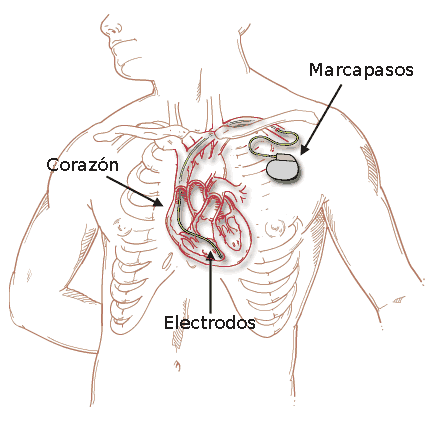
\includegraphics[scale=0.3]{./Introduccion/marcapasos}}
    \subfigure[]{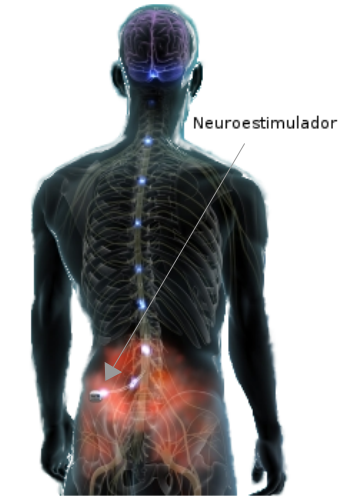
\includegraphics[scale=0.3]{./Introduccion/neuroestimulador}}
    \subfigure[]{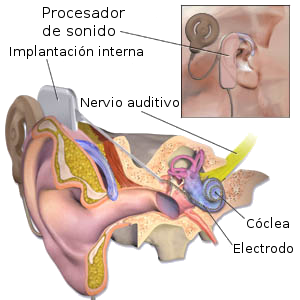
\includegraphics[scale=0.5]{./Introduccion/coclear}}
    \caption{Imágenes de ejemplos de dispositivos médicos implantables. (a) Marcapasos \cite{marcapasos}. (b) Neuroestimulador \cite{neuroestimulador}. (c) Implante coclear \cite{coclear}.}
    \label{fig:fig1.1}
\end{figure}


\section{El sistema de comunicaciones de los dispositivos médicos implantables}\label{sec:enlace}

El uso y tipos de los DMI ha crecido considerablemente desde que en 1958 se implantó el primer marcapasos \cite{brunckhorst}. Desde entonces, los avances en el diseño de los DMI y de sus componentes electrónicos han abierto puertas a funcionalidades más sofisticadas y versátiles. Esta evolución en el diseño de los DMI ha propiciado, a su vez, la posibilidad de configurar las funcionalidades y sus parámetros, pudiendo ser adaptadas a las necesidades de distintos grupos de pacientes.

La configuración de los DMI se realiza a través de un enlace de comunicaciones que pone en contacto al DMI con otro aparato externo. La comunicación del DMI no sólo sirve para programarlo, sino que además suele utilizarse para que el propio dispositivo envíe información recogida por él mismo para procesarla o cualquier otra medida que se lleve a cabo. Debido además a la posición del DMI en el interior del cuerpo humano, lo que hace imposible un contacto físico directo, se ha creado este sistema de comunicaciones en los dispositivos que lo necesiten.

Originalmente, el sistema de comunicaciones de estos dispositivos y otros semejantes ha sido llevada a cabo por un enlace inductivo~\cite{webster,cavuoto}. Sin embargo, este enlace inductivo presenta varias limitaciones: una de ellas es que se debe mantener el dispositivo externo al paciente a muy corta distancia e incluso perfectamente alineado con el DMI; otra limitación es que la capacidad de transferencia de datos es muy baja. Al cabo del tiempo y gracias a los avances arriba mencionados, se ha recurrido al uso de nuevas tecnologías de radiofrecuencia. Estas tecnologías de radiofrecuencia poseen ventajas muy importantes respecto al enlace inductivo: el ancho de banda es mayor (con lo que se puede transmitir y recibir mayor información a una tasa también mayor) y la onda electromagnética transmitida llega más lejos y se atenúa menos, es decir, permite que la comunicación entre el DMI y otro dispositivo sea a mayor distancia. En el capítulo \ref{ch:cap3}, se describen con detalle las tecnologías de radiofrecuencia utilizadas hoy en día para los DMI.

El punto de unión entre los DMI y este Proyecto Fin de Carrera son las antenas que poseen los sistemas de comunicación de estos dispositivos. Estas antenas cumplen una función muy importante, que es la de permitir la comunicación del DMI con otro aparato externo para, como se ha comentado anteriormente, configurar el DMI o recoger información monitorizada del cuerpo o zona del cuerpo donde se ha implantado el dispositivo. El diseño de las antenas debe obedecer varias restricciones impuestas por las características del DMI: deben ser antenas pequeñas, para que puedan ser ubicadas dentro del DMI y que no ocupen mucho espacio; deben ser también antenas eficientes y de bajo consumo, para evitar que el DMI sea reemplazado periódicamente por agotamiento de la batería instalada en el dispositivo y deben ser biocompatibles.

Es por estas razones que hoy en día, el sistema de comunicaciones de los DMI dentro del campo de investigación acutal, sea desarrollado con \textit{antenas microstrip}. Las antenas microstrip fabricadas de manera \textit{embebida}, es decir, fabricadas junto a otros dispositivos, han sido utilizadas por muchas aplicaciones. Destacamos como por ejemplo la aplicación de red de sensores (sensores de movimiento, sensores de humedad, geológicos, etc.) o aplicaciones para la comunicación inalámbrica entre dispositivos, ya sea un teléfono móvil, un GPS, etc~\cite{garg1}. Existen también aplicaciones terapéuticas como es el caso del tratamiento de la hipotermia\footnote{Descenso involuntario de la temperatura corporal por debajo de los 35ºC.} y la hipertermia\footnote{Aumento de la temperatura corporal por encima de los 38ºC; también conocido como \textit{golpe de calor}.} o en uso de catéteres cardíacos~\cite{yang1}. Debido a sus características, que se desarrollan en profundidad en el capítulo~\ref{ch:contexto}, las antenas microstrip son apropiadas para los DMI y su enlace de comunicaciones. Hoy en día son un continuo objeto de estudio por parte de laboratorios de investigación, universidades y empresas ya que son una herramienta muy útil y eficiente para el entorno en el que se desarrolla este Proyecto Fin de Carrera. En el capítulo~\ref{ch:contexto} se proporciona una revisión de trabajos previos de antenas microstrip para DMI.


\section{Objetivos del Proyecto Fin de Carrera}\label{sec:objetivos}

Este Proyecto Fin de Carrera se enmarca dentro del campo de las antenas microstrip para DMI. El \textbf{objetivo global} de este PFC es:

\begin{itemize}

    \item Estudiar, analizar y caracterizar una antena microstrip propuesta en un artículo de la literatura revisada para los sistemas de comunicaciones de los DMI \cite{soont}.
\end{itemize}

\clearpage

\begin{flushleft}
    Otros \textbf{objetivos parciales} recogidos en el proyecto son:
\end{flushleft}

\begin{itemize}
    \item Estudiar la tecnología microstrip, su funcionalidad, ventajas, desventajas y aplicaciones;
    \item Analizar los distintos métodos numéricos de análisis de antenas existentes y en concreto, para las antenas microstrip;
    \item Conocer las propiedades electromagnéticas de los tejidos humanos;
    \item Realizar una revisión bibliográfica de las antenas microstrip, en particular, artículos de investigación actual de antenas microstirp para DMI;
\end{itemize}


\section{Estructura del Proyecto Fin de Carrera}\label{sec:contenidos}

El recorrido por este Proyecto Fin de Carrera está compuesto por cinco capítulos principales:

\begin{itemize}
    \item En el \textbf{Capítulo \ref{ch:contexto} \textit{Contexto tecnológico de las antenas microstrip}}, se presentan las características principales de las antenas microstrip, en especial, las antenas rectangulares. Podemos ver los distintos tipos de análisis teóricos que existen para las mismas, además de sus modos de alimentación. Algunas aplicaciones para DMI se describen al final del capítulo.
    \item En el \textbf{Capítulo \ref{ch:cap3} \textit{Propiedades y modelos electromagnéticos del cuerpo humano y bandas de frecuencia}}, se analizan las distintas propiedades de los tejidos humanos o animales, los modelos de estudio para el cuerpo humano y por último las bandas de frecuencias utilizadas para los DMI.
    \item En el \textbf{Capítulo \ref{ch:metodos} \textit{Metodología}}, se introducen las distintas herramientas que han sido utilizadas en este Proyecto Fin de Carrera.
    \item En el \textbf{Capítulo \ref{ch:simulaciones} \textit{Simulaciones de antenas microstrip en forma de serpentina}}, se entra de lleno en la parte de la simulación de la antena propuesta y distintas variantes a la misma. Estudiamos los distintos parámetros de la antena como son el parámetro $S_{11}$, los campos eléctricos y el diagrama de radiación.
    \item En el \textbf{Capítulo \ref{conclusiones} \textit{Conclusiones y líneas futuras}}, se describen los objetivos conseguidos en este Proyecto Fin de Carrera y las conclusiones finales. Las líneas futuras que se han ido mencionando a lo largo de este texto, quedan recogidas aquí.
    \item En el \textbf{Apéndice I. Presupuesto} se muestra un cálculo aproximado de las horas trabajadas en este Proyecto Fin de Carrera.
    \item En el \textbf{Apéndice II. Artículo wiki} se menciona el aporte extra que acompaña a esta memoria, un artículo wiki alojado en la web del departamento de TSC de la URJC.
\end{itemize}
